\section{Problem Statement}

Cloud computing is a computing model offering a network of PMs to their 
clients in a on-demand fashion. From NIST's definition \cite{Mell:2011jj}, \textit{"cloud computing is a model for enabling ubiquitous, convenient, on-demand network access to a shared pool of configurable computing resources (e.g., networks, PMs, storage, applications and services) that can be rapidly provisioned and released with minimal management effort or service provider interaction."} 
To illustrate how it works, considering a case: a Cloud provider builds a data center which contains thousands of servers connected with network. These servers are virtualized which means they are partitioned into a smaller unit of resources called \emph{Virtual Machines (VMs)}. A web-based application provider can access and deploy their applications (e.g Endnote, Google Drive and etc.) in these VMs from anywhere in the world. Once the applications start serving, application users can use them without installing on their local computers. 

One of the major characteristic of Cloud computing is to separates the role of traditional service provides into Cloud user (software provider) and Cloud (infrastructure) provider. As Wei \cite{Wei:2010fn} states, ``one provides the computing of services, and the other provides the services of computing''. Therefore, stakeholders of Cloud computing become: Cloud providers, Cloud users, and End (application) users \cite{Jennings:2015ht} (see Figure \ref{fig:stakeholders}). This separation beneficial for both Cloud user and End user: It releases the burden of purchasing and maintaining hardwares for Cloud users. Consequently, lower the expense of End users. 

\begin{figure}[H]
	\centering
	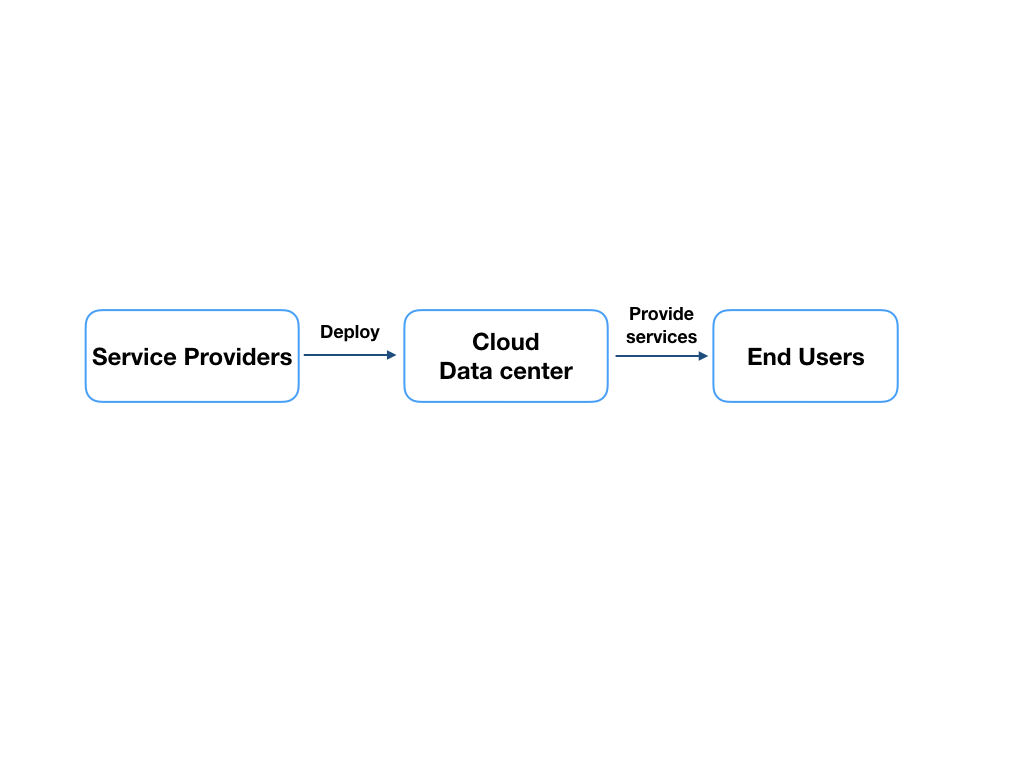
\includegraphics[width=0.7\textwidth]{pics/stakeholders.png}
	\caption{Stakeholders of Cloud computing}
	\label{fig:stakeholders}
\end{figure}
Each stakeholder has their responsibility, goal, and objectives. 
\begin{itemize}
	\item \emph{Cloud providers} build data centers, provide maintenance and resource management on the hardware infrastructure. Their goal is to increase the profit by boosting the income and reducing the expense. Their income comes from Cloud users' rental of servers or \emph{Physical Machines (PMs)} in terms of resource quality (e.g  3.5GHz dual-core CPU), resource quantity (e.g 3 PMs), and time (e.g 1 year). Therefore, Cloud providers objective is to maximize utilization of computing resources. A high utilization brings two benefits, firstly, it increases income by accommodating more applications in limited resources. Secondly, it cuts the expense of energy consumption by packing applications in a minimum number of servers so that idle servers can be turned off. 	
	\item \emph{Cloud users} develop and deploy applications on Cloud. Each application generates time-vary CPU utilization. Their goal is also increase the profit mainly through two objectives, attracting more End users and reduce the expense of resources. The first objective can be achieved by improving the quality of service as well as lower the fee for End users. Either way depends not only on the software entities but also the quality of service (QoS) offered by Cloud provider. The second objective can be achieved by a good estimation of the reserved resources, so that they do not rent insufficient resources which cause low QoS or rent too much resources which cause wastage.
	\item \emph{End Users} are the final customers in this chain. They consume services directly from Cloud users and indirectly from Cloud provider. Their goal is to obtain a satisfactory service. Their goal is achieved by signing a Service Level Agreement (SLA) with Cloud users which constrains the behavior of  the services.
\end{itemize}

In this proposal, we focus on Cloud providers' perspective which is to reduce the energy consumption in Cloud data centers by providing a series of methods to improve the overall resource utilization.

Besides the stakeholders of Cloud computing, Cloud computing has three service models \cite{Mell:2011jj} (see Figure \ref{fig:service_models}): Infrastructure as a Service (IaaS), Platform as a Service (PaaS) and Software as a Service (SaaS). 
Each service model describes distinct responsibilities of stakeholders and the resource management strategies are also different.

\begin{figure}[H]
	\centering
	\begin{subfigure}[b]{0.45\textwidth}
		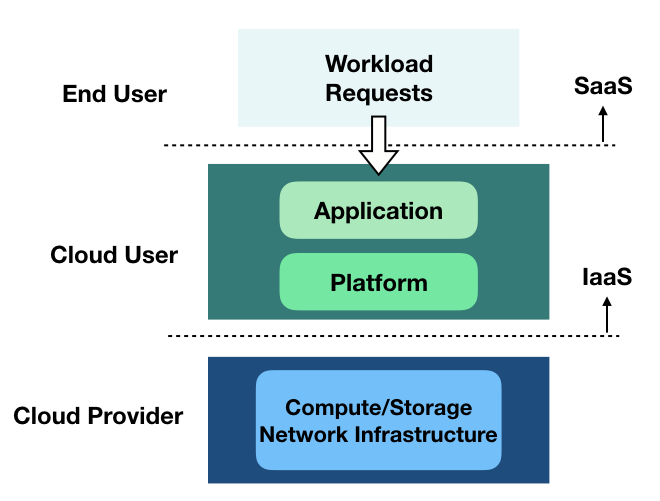
\includegraphics[width=\textwidth]{pics/iaas.png}
		\caption{}
	\end{subfigure}
	\begin{subfigure}[b]{0.45\textwidth}
		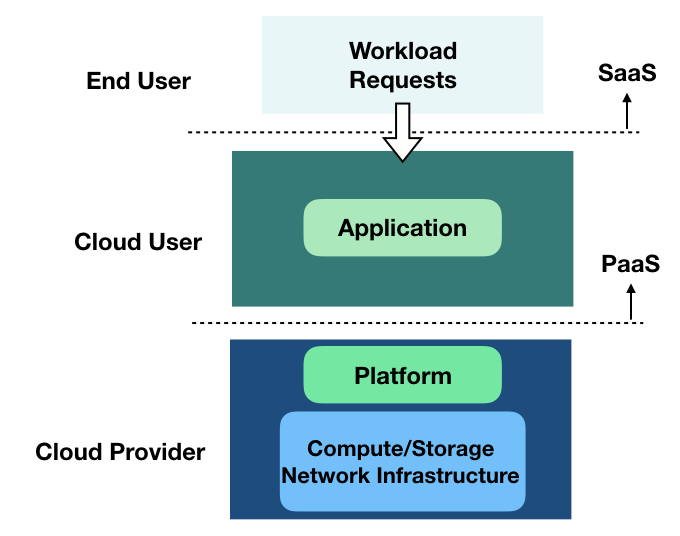
\includegraphics[width=\textwidth]{pics/paas.png}
	\caption{}
	\end{subfigure}
	\caption{Three Service models}
	\label{fig:service_models}
\end{figure}

\begin{itemize}
 	\item \emph{IaaS}, Cloud provider offers the fundamental computing resources, often in the form of various sizes of VMs. Apart from the virtualized hardware and operating systems, Cloud users treat the remote VMs as local and deploy their applications. In terms of resource management, Cloud users have the responsibility to estimate the quantity of resources, while Cloud providers have no knowledge and control inside VMs, resource management is based on VM. 
  	
  	\item \emph{PaaS}, Cloud providers establish the software development platform to enable the in-progress software to be developed in the platform.  The main difference between PaaS and IaaS is that, in PaaS, Cloud providers have the full control of resource allocation. Therefore, Cloud users can focus on software development.
  	
  	\item \emph{SaaS} only describes the relationship between Cloud user and End User, therefore, it does not involve with resource management. Cloud users deploy their applications in Cloud which can be accessed by End Users. 
\end{itemize}



Cloud computing has completely reformed the software industry \cite{Buyya:2009ix} by providing three major benefits to Cloud users.
First, Cloud users do not need upfront investment in hardwares (e.g PMs and networking devices) and pay for hardwares' maintenance. 
Second, Cloud users do not need to worry about the limited resources which can obstruct the performance of their services when unexpected high demand occurs. The elastic nature of cloud can dynamic allocate and release resources for a service. In addition, Cloud user can pay as much as the resource under a \emph{pay-as-you-go} policy.
Third, Cloud users can publish and update their applications at any location 
as long as there is an Internet connection. 
These advantages allow anyone or organization to deploy their softwares on Cloud in
a reasonable price. 

\begin{figure}
	\centering
	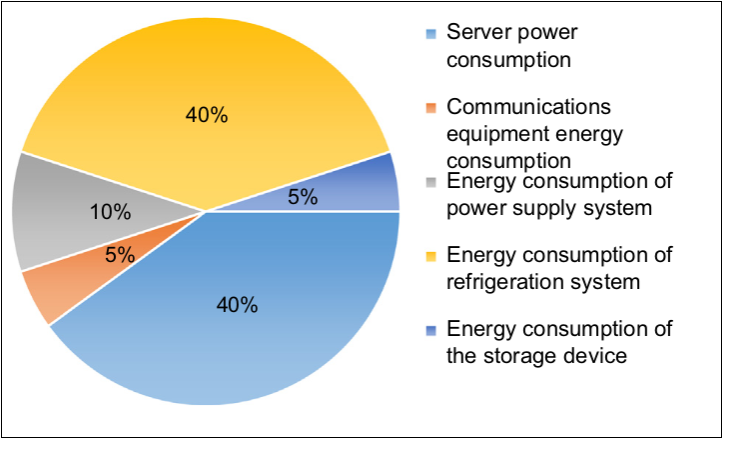
\includegraphics[width=0.5\textwidth]{pics/energyConsumption.png}
	\caption{Energy consumption distribution of data centers \cite{Rong:2016js}}
	\label{fig:consumption}
\end{figure} 

Energy consumption \cite{Kaplan:up01fR-k} is the major concern of Cloud providers. It is derived from several parts as illustrated in Figure \ref{fig:consumption}. 
Regardless the energy consumption of cooling system, 
the majority are from PMs.
According to Hameed et al \cite{Hameed:2016cma}, PMs are far from energy-efficient. 
The main reason for the wastage is that the energy consumption of PMs remains high even when the utilization are low (see Figure \ref{fig:unproportional}). 
Therefore, a concept of \emph{energy proportional computing} \cite{Barroso:2007jt} raised to address the disproportionate between utilization and energy consumption. 
The solution comes two important aspects:  Virtualization technology and resource management strategies. 



\begin{figure}[H]
	\centering
	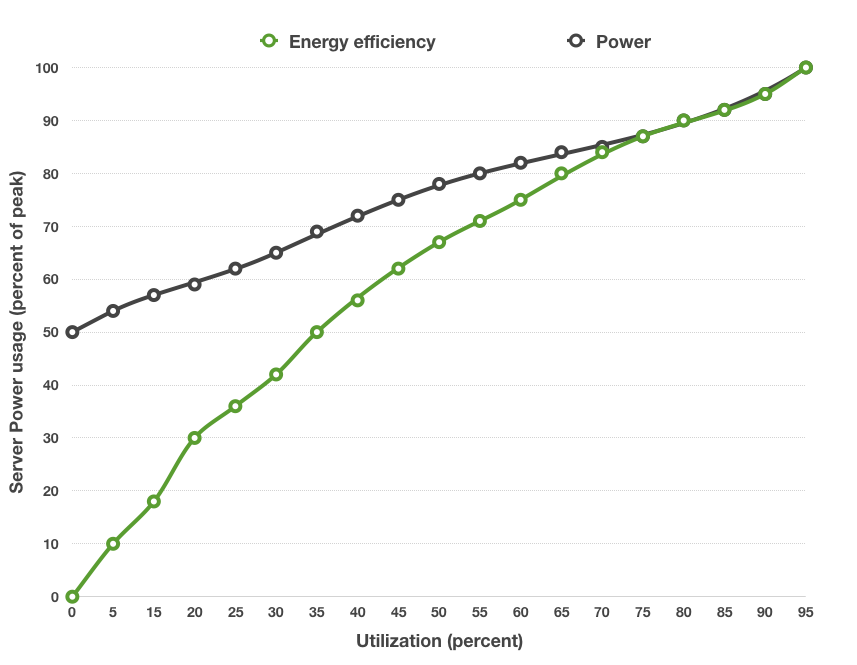
\includegraphics[width=0.5\textwidth]{pics/util.png}
	\caption{Disproportionate between utilization and energy consumption \cite{Barroso:2007jt}}
	\label{fig:unproportional}
\end{figure} 


Virtualization \cite{Uhlig:2005do} is the fundamental technology that enables Cloud computing. It partitions a physical machine's resources (e.g. CPU, memory and disk) into several isolated units called virtual machines (VMs) where each VM allows an operating system running on it. This technology rooted back in the 1960s' and was originally invented to enable isolated software testing. VMs can provide good isolation which means applications running in co-located VMs within the same PM do not interfere each other \cite{Somani:2009ho}.  Soon, people realized that it can be a way to improve the utilization of hardware resources: With each application deployed in a VM, a PM can run multiple applications. Later, a dynamic migration of VM was invented, which compresses and transfers a VM from one PM to another. This technique allows resource management in real time which inspires the strategy of server consolidation. 


Server consolidation \cite{Zhang:2010vo} resolves the low utilization problem by gathering applications into a fewer number of PMs (see Figure \ref{fig:unproportional}), so that the resource utilization of PMs are maintained at a high level and the idle PMs can be turned off to save energy. Consolidation dramatically improves hardware utilization and lowers PM and cooling energy consumption. 


\begin{figure}
	\centering
	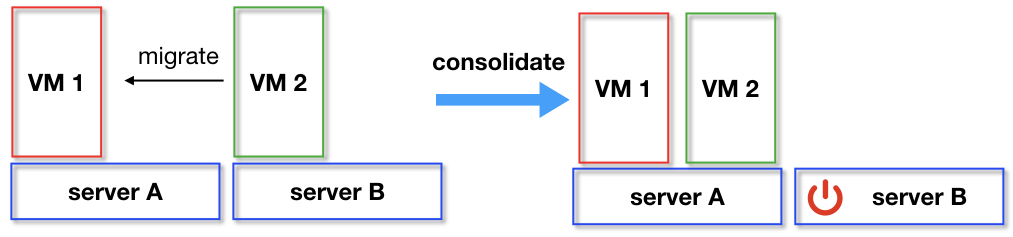
\includegraphics[width=0.7\textwidth]{pics/consolidate.png}
	\caption{A Server Consolidation example: Initially, each PM runs an application wrapped with a VM in a low resource utilization state. After the consolidation, both VMs are running on PM A, so that PM B is turned off to save energy \cite{Barroso:2007jt}.}
	\label{fig:unproportional}
\end{figure} 

Server consolidation is the core functionality involving in all Cloud resource management operations. These operations can be roughly separated into three \cite{Svard:2015ic, Mishra:2012kx} (see Figure \ref{fig:management}) which are applied in different scenarios: Application initialization, Global consolidation, and Dynamic resource management. 

% Data center constantly receives new requests for applications initialization. Once the new applications have been allocated, the utilization begins to drop. This is because, initially, applications are compactly allocated on PMs. As old applications instance are released because of cancelling, the compact structure become loose. Dynamic resource management is a process which can slow the utilization from decreasing. It consolidates by re-allocating one application at a time. Finally, global consolidation is conducted periodically to dramatically improve the resource utilization.
\begin{enumerate}
	\item \emph{Application initialization} is applied when new applications or new VMs arrive and the problem is to allocate them into a minimum number of PMs.

	In this problem, a set of applications or VMs are waiting in a queue. The resource capacity of the PM and usage by applications are characterized by a vector of resource utilizations including CPU, memory and etc. Then, the allocation system must select a minimum number of PMs to accommodate them so that after the allocation, the resource utilizations remain high. The problem is to consider the different combinations of applications so that the overall resource utilization is high. This problem is naturally modeled as a static bin-packing problem \cite{CoffmanJr:1996ui} which is a NP-hard problem meaning it is unlikely to find an optimal solution of a large problem. 

	\item \emph{Global consolidation} is conducted periodically to adjust the current allocation of applications so that the overall utilization is improved.

	In this problem, time is discrete and it can be split into basic time frames, for example: ten seconds. A periodical operation is conducted in every $N$ time frames.
	A cloud data center has a highly dynamic environment with continuous arriving and releasing of applications. Releasing applications cause hollow in PMs; new arrivals cannot change the structure of current allocation. Therefore, after the initial allocation, the overall energy efficiency is likely to drop along with time elapsing. In global consolidation, an optimization system takes the current allocation - including a list of applications/VMs and a list of PMs -  as the input, adjust its allocation so that the global resource utilization is improved.

	In comparison with initialization, instead of new arrivals, the global consolidation considers the previous allocation. Another major difference is that global consolidation needs to minimize the differences of allocation before and after the optimization. This is because the adjustment of allocation relies on a technique called live migration \cite{Clark:2005uda}, and it is a very expensive operation because it occupies the resources in both the host and the target. Therefore, global optimization must be considered as a time-dependent activity which makes the optimization even difficult.

% In comparison with dynamic consolidation, global consolidation takes a set of VMs as input instead of one. Therefore, it is time consuming and often treated as a static problem.
	\item \emph{Dynamic resource management} 
 	Dynamic resource management is applied in three scenarios. \textbf{First},  it is applied when a PM is overloading. Overloading is defined as, one of the resources' consumption exceeds the PM's capacity. At this moment, the applications in that PM are suffering from a Quality of Service (QoS) degradation which means their performance cannot meet the agreement because of the limited resources. Overloading is often caused by the increasing of workload. In order to prevent the QoS from dropping, an application is migrated to another PM. This is called hot-spot mitigation \cite{Mishra:2012kx}. \textbf{Second}, it is applied when a PM is under-loading. Under-loading is when a PM is in a low utilization state normally defined by a threshold. At this moment, all the applications in the under-loading PM are migrated to other active PMs, so the PM becomes empty and can be turned off. This is called dynamic consolidation. \textbf{Third}, it is applied when a PM having very high level of utilization while others having low. An adjustment is to migrate one or more application from high utilized PMs to low ones. This is called load balancing.

	No matter which scenario it is, a dynamic resource management always involves three steps . 
	\begin{itemize}
		\item \emph{When to migrate?} refers to determine the time point that a PM is overloaded or underloaded. It is often decide by a threshold of utilization.
		\item \emph{Which application to migrate?} refers to determine which application need to be migrated so that it optimize the global energy consumption.
		\item \emph{Where to migrate?} refers to determine which host that an application is migrated to. This step is called dynamic placement which is directly related to the consolidation, therefore, it is decisive in improving energy-efficiency. 
	\end{itemize}

	Among three operations, dynamic placement is a dynamic and on-line problem.
	The term ``dynamic'' means the request comes at an arbitrary time point. An on-line problem is a problem which has on-line input and requires on-line output \cite{Borodin:uQcy_H6C}. It is applied when a control system does not have the complete knowledge of future events.

	There are two difficulties in this operation, firstly, dynamic placement requires a fast decision while the search space is very large (e.g hundreds of thousands of PMs). Secondly, migrate one application at a time is hard to reach a global optimized state.

\end{enumerate}

\begin{figure}
	\centering
	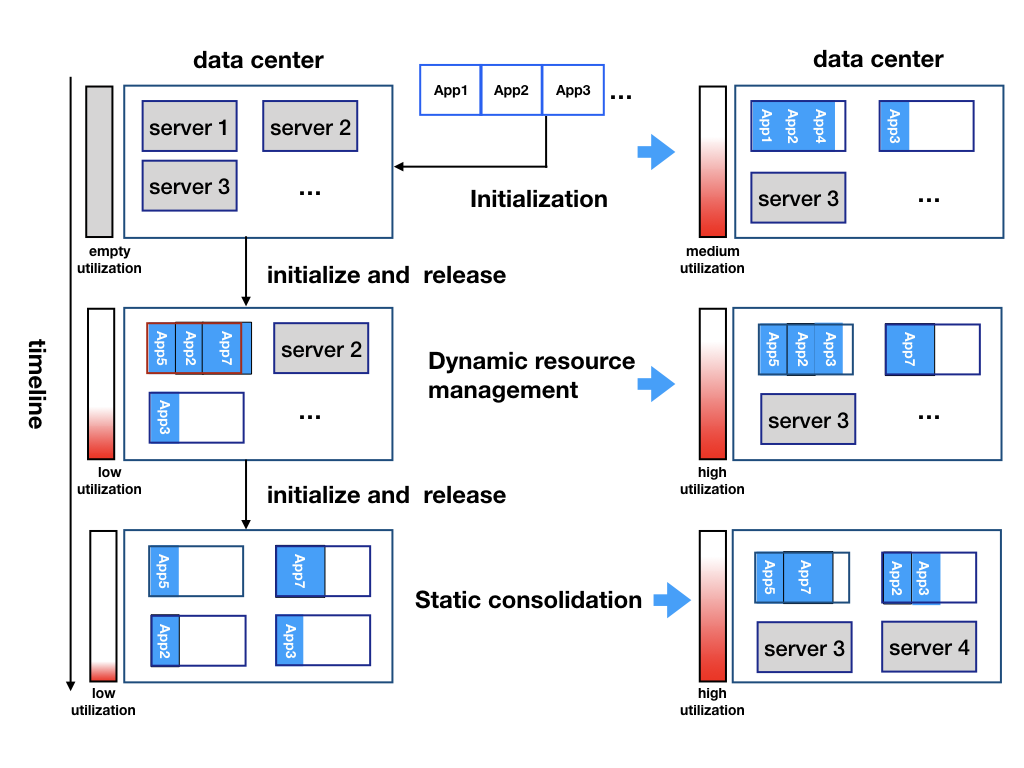
\includegraphics[width=0.8\textwidth]{pics/resource_management.png}
	\caption{Cloud data center resource management involves three steps: initialization, dynamic resource management, and global consolidation. Grey means closed PMs.}
	\label{fig:management}
\end{figure} 

Finally, a consolidation plan includes four major items:
			\begin{enumerate}
				\item A list of existing PMs after consolidation
				\item A list of new virtual machines created after consolidation
				\item A list of old PMs to be turned off after consolidation
				\item The exact placement of applications and services
			\end{enumerate}

By the nature of Cloud resource management, server consolidation techniques can also be categories into static and dynamic methods \cite{Xiao:2015ik, Verma:2009wi}. Static method is a time consuming process which is often conducted off-line in a periodical fashion; initialization and global consolidation belong to this category. It provides a global optimization to the data center. Dynamic method adjusts PMs in real time. It often allocates one application at a time. Therefore, it can be executed quickly and often provides a local optimization to the data center.

\vspace{10mm}
\begin{figure}
	\centering
	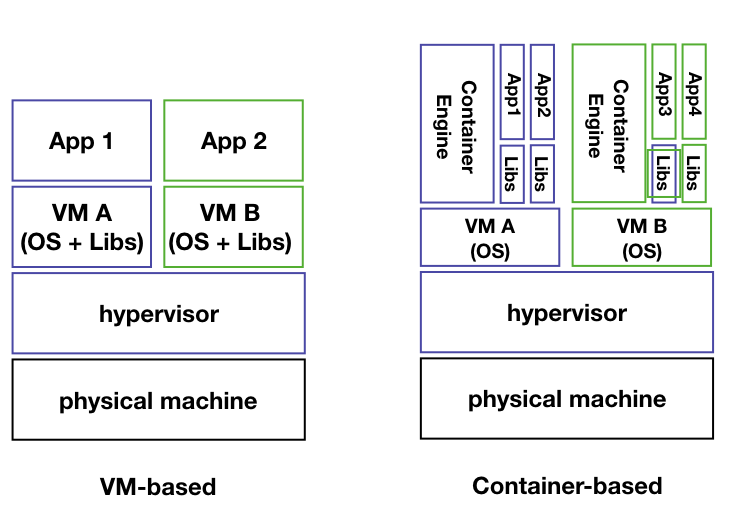
\includegraphics[width=0.7\textwidth]{pics/comparison.png}
	\caption{A comparison between VM-based and Container-based virtualization}
	\label{fig:comparison}
\end{figure}




Besides SaaS which only describes the relationship between Cloud users and End users, PaaS and IaaS have distinct strategies in resource management
In recent years, virtualization technology has evolved to allow finer granularity resource management.
A recent development of Container technique \cite{Soltesz:2007cu} has driven the attention of both industrial and academia.
Container is an operating system level of virtualization which means multiple containers can be installed in a same operating system (see Figure \ref{fig:comparison} right-hand side). Each container provides an isolated environment for an application. In short, a VM is partitioned into smaller manageable units.
This new concept starts a new service model called Container as a Service (CaaS) \cite{Piraghaj:2015uf}. CaaS brings advantages for both Cloud customers and providers.
From Cloud users' perspective, CaaS has advantages of both IaaS (Infrastructure as a Service) and PaaS (Platform as a Service) but without their disadvantages. On one hand - similar to PaaS - it does not require Cloud users to estimate the quantity of resources so that they can focus on application development. On the other hand - similar to IaaS - it allows Cloud users to customize their software environment without being constrained by platforms. 

For Cloud provides, CaaS resolves two IaaS's inherent weaknesses which cause low utilization of resources.
IaaS's weaknesses come from two mechanisms: the separated responsibilities of resource selection for applications and resource allocation; The fixed types of VMs, where each type of VM represents a certain amount of resources (e.g. CPU, RAM, and Storage). 
\begin{itemize}
	\item Firstly, because of separated responsibilities, customers must estimate the quantity of resources. They tend to reserve more resources for ensuring the QoS at the peak hours \cite{Chaisiri:2012cv}. This causes the low utilization.
	\item Secondly, because of the fixed size of VM and the one-on-one mapping of applications and VMs (see Figure \ref{fig:comparison} left hand-side), specific applications consume unbalanced resources which leads to vast amount of resource wastage \cite{Tomas:2013iv}. For example, computation intensive tasks consume much more CPU than RAM; a fixed type of VM provides much more RAM than it needs. Because the tasks use too much CPU, they prevent other tasks from co-allocating.
	This causes wastage.
\end{itemize}

In contrast, CaaS solves above two problems at a time. It allows Cloud providers to manage both the resource selection for applications and resource allocation; It also enables VM-resizing and many-to-one mapping between applications to VMs (Figure \ref{fig:comparison} right hand-side).
Hence, Cloud providers have a complete control of resources which may result in a better utilization of resources. 
In addition, IaaS Cloud runs many redundant operating systems and hypervisors. CaaS eliminates these redundancies by a single operating system with multiple containers.
% do research in this field.

\vspace{10mm}

Currently, vast amount of server consolidation methods are mostly VM-based and they are mainly modeled as bin-packing problems \cite{Mann:2015ua}, where applications represent items and PMs represent bins. These methods can not be directly applied on container-based problem because container-based consolidation has two levels of allocation: Containers are allocated to VM as the first level and VM are allocated to PM as the second level. These two levels of allocation interact with each other. 

Even for single level of bin-packing problems, the complexity is NP-hard .
In VM-based static problem, deterministic methods such as  
Integer Linear Programming \cite{Speitkamp:2010ck} and Mixed
Integer Programming \cite{Wang:2016eh} are often considered. However, it is well-known that they are very time-consuming for a large scale problem. More research proposed heuristic methods
 to approximate the optimal solution such as 
First Fit Decreasing (FFD) \cite{Panigrahy:2011wk}, Best Fit Decreasing (BFD) \cite{Beloglazov:2012ji}.
Manually designed heuristics are designed to tackle the special requirements such 
as a bin-item incomplete scenario \cite{Gupta:2008ul} and multi-tier applications \cite{Jung:2008vb, Li:2009wf}. Although these greedy-based heuristics can quickly approximate an answer,  as Mann's research \cite{Mann:2015ua} showed, server consolidation is a lot more harder than bin-packing problem because of the multi-dimensional, many constraints. Therefore, general bin-packing algorithms do not perform well with many constraints and specific designed heuristics only perform well in very narrow scope.

Evolutionary Computation (EC) is commonly used to solve combinatorial optimization problem \cite{Guzek:2015ds}, therefore, it is particular useful in solving the global consolidation problem.  Many EC techniques including Genetic Algorithm (GA) \cite{Xu:2010vh}, Ant Colony Optimization (ACO) \cite{Gao:2013gg, Mateos:2013bm}, Particle Swarm Optimization (PSO) \cite{Jeyarani:2012fg} have been used in solving this problem. EC algorithms show their advantages in the following aspects. Firstly, EC algorithms are good at solving multi-objective problems because of their population-based nature. And global consolidation problem often involves two or more objectives (e.g energy efficiency and migration cost). Secondly,  they can provide near-optimal solutions within a reasonable amount of time.  

In VM-based dynamic problem, 
previous most research proposed human designed greedy-based dispatching rules or heuristics such as a First-Fit-based approach \cite{Bobroff:2007ec}, Modified Best Fit Decreasing \cite{Beloglazov:2012ji}, and a two-stage heuristic \cite{Zhang:2015jm}. One of the major problem for human designed heuristics is that if any inherent component gets changes, then the designed heuristic may not work as it was expected \cite{SoteloFigueroa:2013be}. EC algorithms are also seldom considered in this scenario because most EC methods need more time to search through solutions space.

Only a few research focus on container-based consolidation, Piraghaj \cite{Piraghaj:2016bw} designs a dynamic allocation system. She proposes a two-step procedure; it first maps tasks to VMs and then allocate containers to VMs. As Mann illustrated in \cite{Mann:2016hx},  these two steps should be conducted simultaneously, otherwise it leads to local optimal. Other research \cite{Dong:2014iz, Hindman:2011ux, Anselmi:2008ik} propose greedy-based heuristics on container allocation problem. They can be easily stuck at local optimal. 
This thesis, therefore, aims at providing an end-to-end solution for Container-based server consolidation which includes three stages correspond with the Cloud resource management procedure (see Figure \ref{fig:management}): initialization, static container-based server consolidation and dynamic container placement.

% Despite the usefulness of server consolidation, it is a difficult task. Traditional server consolidation is conducted manually \cite{Chebiyyam:2009uq} with vast data analysis and interviews with application owners. It is fraught and extremely difficult to reach a global optima state.
% Later on, server consolidation is often considered as a global optimization problem 
% where its goal is to minimize the overall energy consumption. 
% It is often modeled as a bin-packing problem \cite{Mann:2015ua} which is a well-known NP-hard problem meaning it is unlikely to find an optimal solution of a large problem. 

% In static methods, deterministic methods such as  
% Integer Linear Programming \cite{Speitkamp:2010ck} and Mixed
% Integer Programming \cite{Wang:2016eh} are often considered. However, it is well-known that they are very time-consuming for a large scale problem. More research proposed heuristic methods
%  to approximate the optimal solution such as 
% First Fit Decreasing (FFD) \cite{Panigrahy:2011wk}, Best Fit Decreasing (BFD) \cite{Beloglazov:2012ji}.
% Manually designed heuristics are designed to tackle the special requirements such 
% as a bin-item incomplete scenario \cite{Gupta:2008ul} and Multi-tier Applications \cite{Jung:2008vb, Li:2009wf}. Although these greedy-based heuristics can quickly solve the consolidation problem,  as Mann's research \cite{Mann:2015ua} shown, server consolidation is a lot more harder than bin-packing problem because of multi-dimension, many constraints. Therefore, a simple greedy-based heuristic (e.g FFD) leads to a bad performance. 

% Evolutionary Computation (EC) is commonly used to solve combinatorial optimization problem \cite{Guzek:2015ds}, therefore, it is particular useful in solving the global consolidation problem.  Many EC techniques including Genetic Algorithm (GA) \cite{Xu:2010vh}, Ant Colony Optimization (ACO) \cite{Gao:2013gg, Mateos:2013bm}, Particle Swarm Optimization (PSO) \cite{Jeyarani:2012fg} have been used in solving this problem. EC algorithms show their advantages in the following aspects. Firstly, EC algorithms are good at solving multi-objective problems because of their population-based nature. And global consolidation problem often involves two or more objectives (e.g energy efficiency and migration cost). Secondly,  they can provide near-optimal solutions within a reasonable amount of time.  

% Dynamic consolidation problem requires fast decision-making and global optimization. Previous most research proposed human designed greedy-based dispatching rules or heuristics such as a First-Fit-based approach \cite{Bobroff:2007ec}, Modified Best Fit Decreasing \cite{Beloglazov:2012ji}, and a two-stage heuristic \cite{Zhang:2015jm}. One of the major problem for human designed heuristics is that if any inherent component gets changes, then the designed heuristic may not work as it was expected \cite{SoteloFigueroa:2013be}. EC algorithms are also seldom considered in this scenario because most EC methods need more time to search through solutions space.

